\documentclass[output=paper,colorlinks,citecolor=brown
% ,hidelinks
% showindex
]{langscibook}

\ChapterDOI{10.5281/zenodo.12665913}
\author{Iris Berent\orcid{0000-0003-2820-9693}\affiliation{Northeastern University}}
\title{Why is UG such a hard question?}
\abstract{UG presents a hard problem for scholars. Here, I ask why the question of innate rules of language is so difficult to settle. The problem, I suggest, does not lie in the innateness question itself—whether knowledge, of language or otherwise, is innate knowledge, is a perfectly coherent question. And yet, ``innate knowledge'' is a notion that is difficult for us to grasp. New experimental evidence suggests that laypeople are systematically biased to presume that knowledge only arises from experience, and this Empiricist bias is rooted in core cognition (e.g., \cite{berent2022autism}). These results open up the possibility that our troubles with UG arise from this very bias. Whether linguists are indeed biased, and whether these attitudes are anchored in core cognition is unknown. But the possibility that our troubles with UG have innate origins merits close attention.}

\graphicspath{ {./figures/} }
\IfFileExists{../localcommands.tex}{
   \addbibresource{../localbibliography.bib}
   \usepackage{orcidlink}
\usepackage{tabularx,multicol}
\usepackage{url}
\urlstyle{same}

\usepackage{siunitx}
\sisetup{group-digits = none}

\usepackage{langsci-branding} 
\usepackage{langsci-optional}
\usepackage{langsci-lgr}
\usepackage{langsci-tbls}
\usepackage{langsci-gb4e}

% Müller
\usepackage{tikz-qtree}
\usepackage{hologo}

% 3_pullum.tex
\usepackage{langsci-textipa}

% 8_levine
\usepackage{bm}
\usepackage{umoline}
\usepackage{pifont}
\usepackage{pstricks,pst-node,pst-tree}
\usepackage{ulem}
\usepackage{mathrsfs}
\usepackage{bussproofs}

% 14_kornai
\usepackage[matrix,arrow]{xy}
\usepackage{subcaption}

\usepackage[linguistics, edges]{forest}
\usetikzlibrary{arrows, arrows.meta}

   \SetupAffiliations{output in groups = false,
                   orcid placement = after,
                   separator between two = {\bigskip\\},
                   separator between multiple = {\bigskip\\},
                   separator between final two = {\bigskip\\}
                   }

% ORCIDs in langsci-affiliations 
\definecolor{orcidlogocol}{cmyk}{0,0,0,1}
\RenewDocumentCommand{\LinkToORCIDinAffiliations}{ +m }
  {%
    \,\orcidlink{#1}%
  }

\makeatletter
\let\thetitle\@title
\let\theauthor\@author
\makeatother

% Cite and cross-reference other chapters
\newcommand{\crossrefchaptert}[2][]{\citet*[#1]{chapters/#2}, Chapter~\ref{chap-#2} of this volume} 
\newcommand{\crossrefchapterp}[2][]{(\citealp*[#1]{chapters/#2}, Chapter~\ref{chap-#2} of this volume)}
\newcommand{\crossrefchapteralt}[2][]{\citealt*[#1]{chapters/#2}, Chapter~\ref{chap-#2} of this volume}
\newcommand{\crossrefchapteralp}[2][]{\citealp*[#1]{chapters/#2}, Chapter~\ref{chap-#2} of this volume}

\newcommand{\crossrefcitet}[2][]{\citet*[#1]{chapters/#2}} 
\newcommand{\crossrefcitep}[2][]{\citep*[#1]{chapters/#2}}
\newcommand{\crossrefcitealt}[2][]{\citealt*[#1]{chapters/#2}}
\newcommand{\crossrefcitealp}[2][]{\citealp*[#1]{chapters/#2}}


\newcommand{\sub}[1]{\textsubscript{\scriptsize\textrm{#1}}}
% Müller
\newcommand{\page}{}

\let\citew\citet
\def\underRevision{Revise and resubmit}
\let\textbfemph\emph

%% % taken from https://tex.stackexchange.com/a/95079/18561
\newbox\usefulbox

\makeatletter
\def\getslant #1{\strip@pt\fontdimen1 #1}

\def\skoverline #1{\mathchoice
 {{\setbox\usefulbox=\hbox{$\m@th\displaystyle #1$}%
    \dimen@ \getslant\the\textfont\symletters \ht\usefulbox
    \divide\dimen@ \tw@ 
    \kern\dimen@ 
    \overline{\kern-\dimen@ \box\usefulbox\kern\dimen@ }\kern-\dimen@ }}
 {{\setbox\usefulbox=\hbox{$\m@th\textstyle #1$}%
    \dimen@ \getslant\the\textfont\symletters \ht\usefulbox
    \divide\dimen@ \tw@ 
    \kern\dimen@ 
    \overline{\kern-\dimen@ \box\usefulbox\kern\dimen@ }\kern-\dimen@ }}
 {{\setbox\usefulbox=\hbox{$\m@th\scriptstyle #1$}%
    \dimen@ \getslant\the\scriptfont\symletters \ht\usefulbox
    \divide\dimen@ \tw@ 
    \kern\dimen@ 
    \overline{\kern-\dimen@ \box\usefulbox\kern\dimen@ }\kern-\dimen@ }}
 {{\setbox\usefulbox=\hbox{$\m@th\scriptscriptstyle #1$}%
    \dimen@ \getslant\the\scriptscriptfont\symletters \ht\usefulbox
    \divide\dimen@ \tw@ 
    \kern\dimen@ 
    \overline{\kern-\dimen@ \box\usefulbox\kern\dimen@ }\kern-\dimen@ }}%
 {}}
\makeatother

% 1_intro.tex

% For the block quote:
\definecolor{linequote}{RGB}{224,215,188}
\definecolor{backquote}{RGB}{249,245,233}

\NewDocumentEnvironment{myquote}{ +m }
  {%
    \begin{tblsfilled}{}[black!12]
    #1%
  }
  {\end{tblsfilled}}

% 2_gibson.tex


% Example(s) Environments
% 12pt, No new-lines after example number is printed

\newcounter{examplectr}
\newcounter{fnexamplectr}

% Note: don't use subexamples in footnotes.

% This line is to overcome a bug in cmu-art style: it prints counter
% values to the aux file using \theaux... rather than using \the...
\def\theauxexamplectr{\theexamplectr}

\newcounter{subexamplectr}
\def\theauxsubexamplectr{\thesubexamplectr}
\def\theauxfnexamplectr{\thefnexamplectr}

\renewcommand{\theexamplectr}{\arabic{examplectr}}
% This command causes example numbers to appear without following periods

\renewcommand{\thefnexamplectr}{\roman{fnexamplectr}}
% This command causes example numbers to appear without following periods

\renewcommand{\thesubexamplectr}{\theexamplectr\alph{subexamplectr}}
% This command gives the number of an example and subexample as e.g. 1a, 2b

\newlength{\wdth}
\newcommand{\strike}[1]{\settowidth{\wdth}{#1}\rlap{\rule[.5ex]{\wdth}{1pt}}#1}

\newcommand{\exref}[1]{(\ref{#1})}
% This command puts reference numbers with parentheses
% surrounding them 

% The environment ``examples'' gives a list of examples, one on each line,
% numbered with a lower case alphabetic character
\newenvironment{examples}%
   { \vspace{-\baselineskip}
     \begin{list}%
     \textrm{\alph{subexamplectr}.}%
     {\usecounter{subexamplectr}
     \setlength{\topsep}{-\parskip}
     \setlength{\itemsep}{-2pt}
     \setlength{\leftmargin}{0.5in}
     \setlength{\rightmargin}{0in} } }%
   { \end{list}}

% The environment ``myexample'' outputs an arabic counter ``examplectr''
% surrounded by parentheses.
\newenvironment{myexample}
   { \vspace{20pt}
     \noindent
     \begin{minipage}{\textwidth}    % minipage environment disallows
                 % breaks across pages

     \refstepcounter{examplectr}     % step the counter and cause this
                 % section to be referenced by the
                 % counter ``examplectr''
     (\arabic{examplectr})}%
   { \vspace{20pt}
     \end{minipage}}

\newenvironment{myfnexample}
   { \vspace{2pt}
     \noindent
     \begin{minipage}{\textwidth}    % minipage environment disallows
                 % breaks across pages

     \refstepcounter{fnexamplectr}     % step the counter and cause this
                 % section to be referenced by the
                 % counter ``examplectr''
     (\roman{fnexamplectr})}%
   { \vspace{2pt}c
     \end{minipage}}
    
\newcommand*\circled[1]{\tikz[baseline=(char.base)]{
            \node[shape=circle,draw,inner sep=2pt] (char) {#1};}}

\newcommand{\data}[1]{\textit{#1}}
\newcommand{\nodata}[1]{#1}
\newcommand{\blank}{\rule{1.2em}{0.5pt}}
\newcommand{\pt}[1]{\ensuremath{\mathsf{#1}}}
\newcommand{\ptv}[1]{\ensuremath{\textsf{\textsl{#1}}}}
\newcommand{\sv}[1]{\ensuremath{\mathcal{#1}}}

\newcommand{\sX}{\sv{X}}
\newcommand{\sF}{\sv{F}}
\newcommand{\sG}{\sv{G}}
\newcommand{\greekp}{\upvarphi}
\newcommand{\greekr}{\uprho}
\newcommand{\greeks}{\upsigma}
\newcommand{\MultiLine}[1]{\ensuremath{\begin{array}[b]{@{}l@{}}#1\end{array}}}
\newcommand{\LexEnt}[3]{#1; \ensuremath{#2}; \syncat{#3}}

\newcommand{\LexEntBroken}[3]
  {\Shortstack
      {%
        {#1;} 
        {\ensuremath{#2};} 
        {\syncat{#3}}%
      }%
  }

\newcommand{\grey}[1]{\colorbox{mycolor}{#1}}
\definecolor{mycolor}{gray}{0.8}

\newcommand{\gap}{\longrule}
\newcommand{\gp}{\gap}
\newcommand{\vs}{\raisebox{.05em}{\ensuremath{\,\upharpoonright}}}

\newcommand{\E}{ε}

\newcommand{\EBob}[1]{\textsl{#1}}

\newcommand{\B}{\textbf}
\newcommand{\f}{{\color{green}f}}  % Question what does f do? It does not have any output in the
                                % original PDF
%\newcommand{\Lemma}{{\color{pink}Lemma}}
\newcommand{\Lemma}{\ensuremath{\vdots\hskip.5cm\vdots}\noLine}

%\newcommand{\calP}{{\color{pink}calP}} % Sebastian
\newcommand{\calP}{\ensuremath{\mathcal{P}}}


\newcommand{\maru}[1]{\ooalign{\hfil#1\/\hfil\crcr
      \raise.05ex\hbox{\LARGE\mathhexbox20D}}}


%\newcommand{\sem}[2][M\!,g]{\mbox{$[\![ \mathrm{#2} ]\!]^{#1}$}}
\newcommand{\sem}{\ensuremath}

%
\newcommand{\trns}[1]{\textbf{#1}\xspace}
\newcommand{\bs}{{\textbackslash}}
\newcommand{\bsl}{{\bs}}
\newcommand{\fb}[1]{\textsubscript{#1}}
\newcommand{\syncat}[1]{\ensuremath{\mathrm{#1}}}
\newcommand{\term}[1]{\textit{#1}}
\newcommand{\LemmaAlt}{\ensuremath{\vdots\hskip.5cm\vdots}}
\NewDocumentCommand{\VanLabel}{m}{\MakeUppercase{#1}}

   %% hyphenation points for line breaks
%% Normally, automatic hyphenation in LaTeX is very good
%% If a word is mis-hyphenated, add it to this file
%%
%% add information to TeX file before \begin{document} with:
%% %% hyphenation points for line breaks
%% Normally, automatic hyphenation in LaTeX is very good
%% If a word is mis-hyphenated, add it to this file
%%
%% add information to TeX file before \begin{document} with:
%% %% hyphenation points for line breaks
%% Normally, automatic hyphenation in LaTeX is very good
%% If a word is mis-hyphenated, add it to this file
%%
%% add information to TeX file before \begin{document} with:
%% \include{localhyphenation}
\hyphenation{
    Ber-ti-net-to
    caus-a-tive
    fest-schrift
    Fest-schrift
    Hix-kar-ya-na
    In-do-ne-sian
    mor-pho-phon-o-log-i-cal
    Mo-se-tén
    par-a-digm
    phra-ses
    Que-chua
}

\hyphenation{
    Ber-ti-net-to
    caus-a-tive
    fest-schrift
    Fest-schrift
    Hix-kar-ya-na
    In-do-ne-sian
    mor-pho-phon-o-log-i-cal
    Mo-se-tén
    par-a-digm
    phra-ses
    Que-chua
}

\hyphenation{
    Ber-ti-net-to
    caus-a-tive
    fest-schrift
    Fest-schrift
    Hix-kar-ya-na
    In-do-ne-sian
    mor-pho-phon-o-log-i-cal
    Mo-se-tén
    par-a-digm
    phra-ses
    Que-chua
}

   \boolfalse{bookcompile}
   \togglepaper[23]%%chapternumber
   \graphicspath{ {../figures/} }
}{}

   
\begin{document}
\maketitle

\noindent I am very pleased to offer this essay in celebration of the life and work of Dan Everett. Dan was my linguistics professor at Pitt. Although he was not my advisor, nor was linguistics my major, Dan left a lasting mark on my intellectual development. With his inexhaustible fervor, sharp wit and piercing questions, the redhead professor left us students in awe, silent, dazzled, and a bit frightened. 

What was so impressive about Dan wasn’t his command of formal theories (at the time, it was autosegmental phonology) -- those theories come and go. Rather, Dan saw language as a window into human nature, and he invited us, students, to lean forward and take a peek. So, it is only befitting that, in tribute to my teacher, I broach that subject here.

The topic of my piece is Universal grammar (UG) --  the hypothesis that the human capacity for language arises from innate knowledge of linguistic principles \citep{chomsky1965aspects}. Since UG concerns what’s innate in humans, it addresses human nature.  But as Dan explained at the time, UG articulates a well-defined scientific hypothesis that is amply amenable to empirical scrutiny.\footnote{The question of ``innate knowledge'' as discussed here, is amply amenable to empirical scrutiny. As such, the ``innateness question'' is distinct from the debate regarding merits of Rationalism as a method of inquiry (in philosophy, Rationalism has been frequently invoked to argue for a priori knowledge).} And yet, nearly sixty years past Chomsky’s \textit{Aspects} \citep{chomsky1965aspects}, the question of whether UG exists (hereafter: the UG question) remains as contentious as ever.  Arguably, it’s one of the hardest questions in cognitive science.

In this piece, I won’t take sides on the UG debate, and I certainly won’t seek to settle it.  My goal is not to determine whether innate knowledge of language exists. Rather, I ask why the UG question is so difficult for science to settle.  

To foreshadow my conclusions, I don’t believe that the problem is with the notion of innateness nor do I think the problem is specific to the inquiry into ``innate knowledge of language''. Rather, I suggest that the problem is with the inquirer.  

Supported by recent experimental findings from my lab, I will show that humans are systematically biased in their reasoning about all forms of innate knowledge, UG included. It is these biases, I believe, that render UG a particularly difficult question.

\section{``Innateness'' is a perfectly coherent question!}
Doing science is hard -- that much goes without saying. But questions about the mind, especially those concerning innateness, are extra difficult. Debates about innateness just don’t go away, and this can be frustrating. For some, the question of innateness seems incoherent \citep{mameli2011evaluation}. 

I don’t think it is. Cognitive innateness, of course, does not lend itself to definition by a set of necessary and sufficient conditions. But so do many other human concepts. And yet, we use such concepts in science, and make good progress. The fact that ``game'', for instance, cannot be defined \citep{wittgenstein1953philosophical} has hardly stopped the blooming field of game theory (e.g., \cite{nowak1999evolution}).  So, I don’t think our troubles with innateness arise from the lack of definitions.\largerpage

Concerns with innateness also cannot be obviated by the insights from genetics. Critics note that genes and environment interact, and this of course is true of all biological traits (e.g., \cite{ridley2003nature}). Still, some biological traits emerge spontaneously among members of the species (e.g., having two hands) and others (e.g., a scratch, a severed limb) do not. It is perfectly coherent to ask whether a given trait is largely heritable -- is it more like having two hands or a scratch?

To make progress, however, questions about innateness ought to be formulated at a specific level of analysis \citep{samuels2004innateness}. Although we all agree that having two hands is an innate feature of humans, this trait (like all others) develops; the human zygote obviously has no hands, yet all healthy human embryos do. 
By the same token, UG is a cognitive trait, so when we consider its innateness, we ought to explicate it within the cognitive level of analysis. As \citet{samuels2004innateness} notes, some cognitive traits are the product of cognitive mechanisms, whereas other cognitive traits are not -- they are cognitive primitives. The knowledge that ``Paris is the capital of France'' is obviously the product of learning, but other concepts, such as what is an ``object'', arguably aren’t and, as such, are good candidates for ``cognitive primitives''. Innate cognitive traits, then, are cognitive primitives; these are cognitive traits that emerge spontaneously in the normal course of development, but they are not the product of other cognitive mechanisms.

Viewed in this manner, the UG question is straightforward: is UG a cognitive primitive, or does it emerge from other cognitive mechanisms -- most notably, learning from experience?
The answer can be either ``yes'' or ``no'' -- either UG exists, or it doesn’t. But there is nothing wrong with asking: the question is logically coherent. 

And yet, the notion of UG strikes us as ``funny'' -- it doesn’t quite ``compute''. But, as we will see next, that sense of unease applies to the notion of innate knowledge, generally -- it is not specific to UG. ``Innate knowledge'' is a notion that is extremely difficult for people to comprehend. The concept of innate knowledge~-- of any kind -- simply strikes people as an oxymoron.

\section{Innate knowledge -- what a ``funny'' notion!}

When laypeople -- adults and children -- are asked to evaluate the origins of knowledge, they are systematically biased to assume that knowledge arises from experience. This is the case across multiple instances of knowledge, across multiple manners of probing, and when people consider knowledge of different creatures -- humans, animals and even aliens \citep{berent2019people,wang2019empiricism}.

For example, when asked to evaluate which psychological trait would likely emerge among infants who are raised on a ``desert island'', people assert that knowledge will not emerge spontaneously, even when the notions in question are ones that have been documented across cultures, and thus, plausibly innate (e.g., ``keeping track of time'', ``logical negation''; \cite{berent2019people}). The same is obtained when people are asked about the knowledge of infants (e.g., that objects are cohesive) and animals (e.g., the structure of a swamp sparrow’s song), and when innateness is gauged indirectly, by asking people to predict the onset of traits in development \citep{berent2019people}. People reject that knowledge is innate, and they tend to believe it emerges late in development, even when the traits in question are demonstrably present in young infants or at birth \citep{wang2019empiricism}.

This is not because people uniformly reject all forms of innateness. In fact, when asked the same about other aspects of the psyche -- about sensations, motor skills and emotions -- people have no problem assuming that these capacities are innate and early emerging \citep{berent2019people}. In fact, they are positively biased to assume that emotions are innate, and they manifest this bias even when they are explicitly told that the emotions in question are learned \citep{berent2020essentialist}. It is specifically the notion of innate knowledge, then, that seems ``funny''. And this is also demonstrably so when people are asked about innate knowledge of language.

In one study, we asked people to weigh in on the origins of language structure \citep{berent2019people}. Participants were presented with two matched vignettes (\figref{fig:figure1a}; emphases are added). Each such vignette presented an explanation for linguistic structure. One explanation attributed structure (specifically, syntax) to abstract rules (simplified, for the lay readers); another attributed structure (syllable structure) to articulatory pressures.  In both cases, people were told that the structural regularity in question develops spontaneously, without learning (i.e., innate). Next, we asked participants to evaluate whether these traits will emerge in a ``desert island'' scenario -- among a group of children that are fully cared for, but have had no opportunity to observe language in others. People considered syntactic rules as less likely to be innate (i.e., to emerge spontaneously) than articulatory motor plans (\figref{fig:figure1b}). 

\begin{figure}
    \begin{subfigure}{\textwidth}
    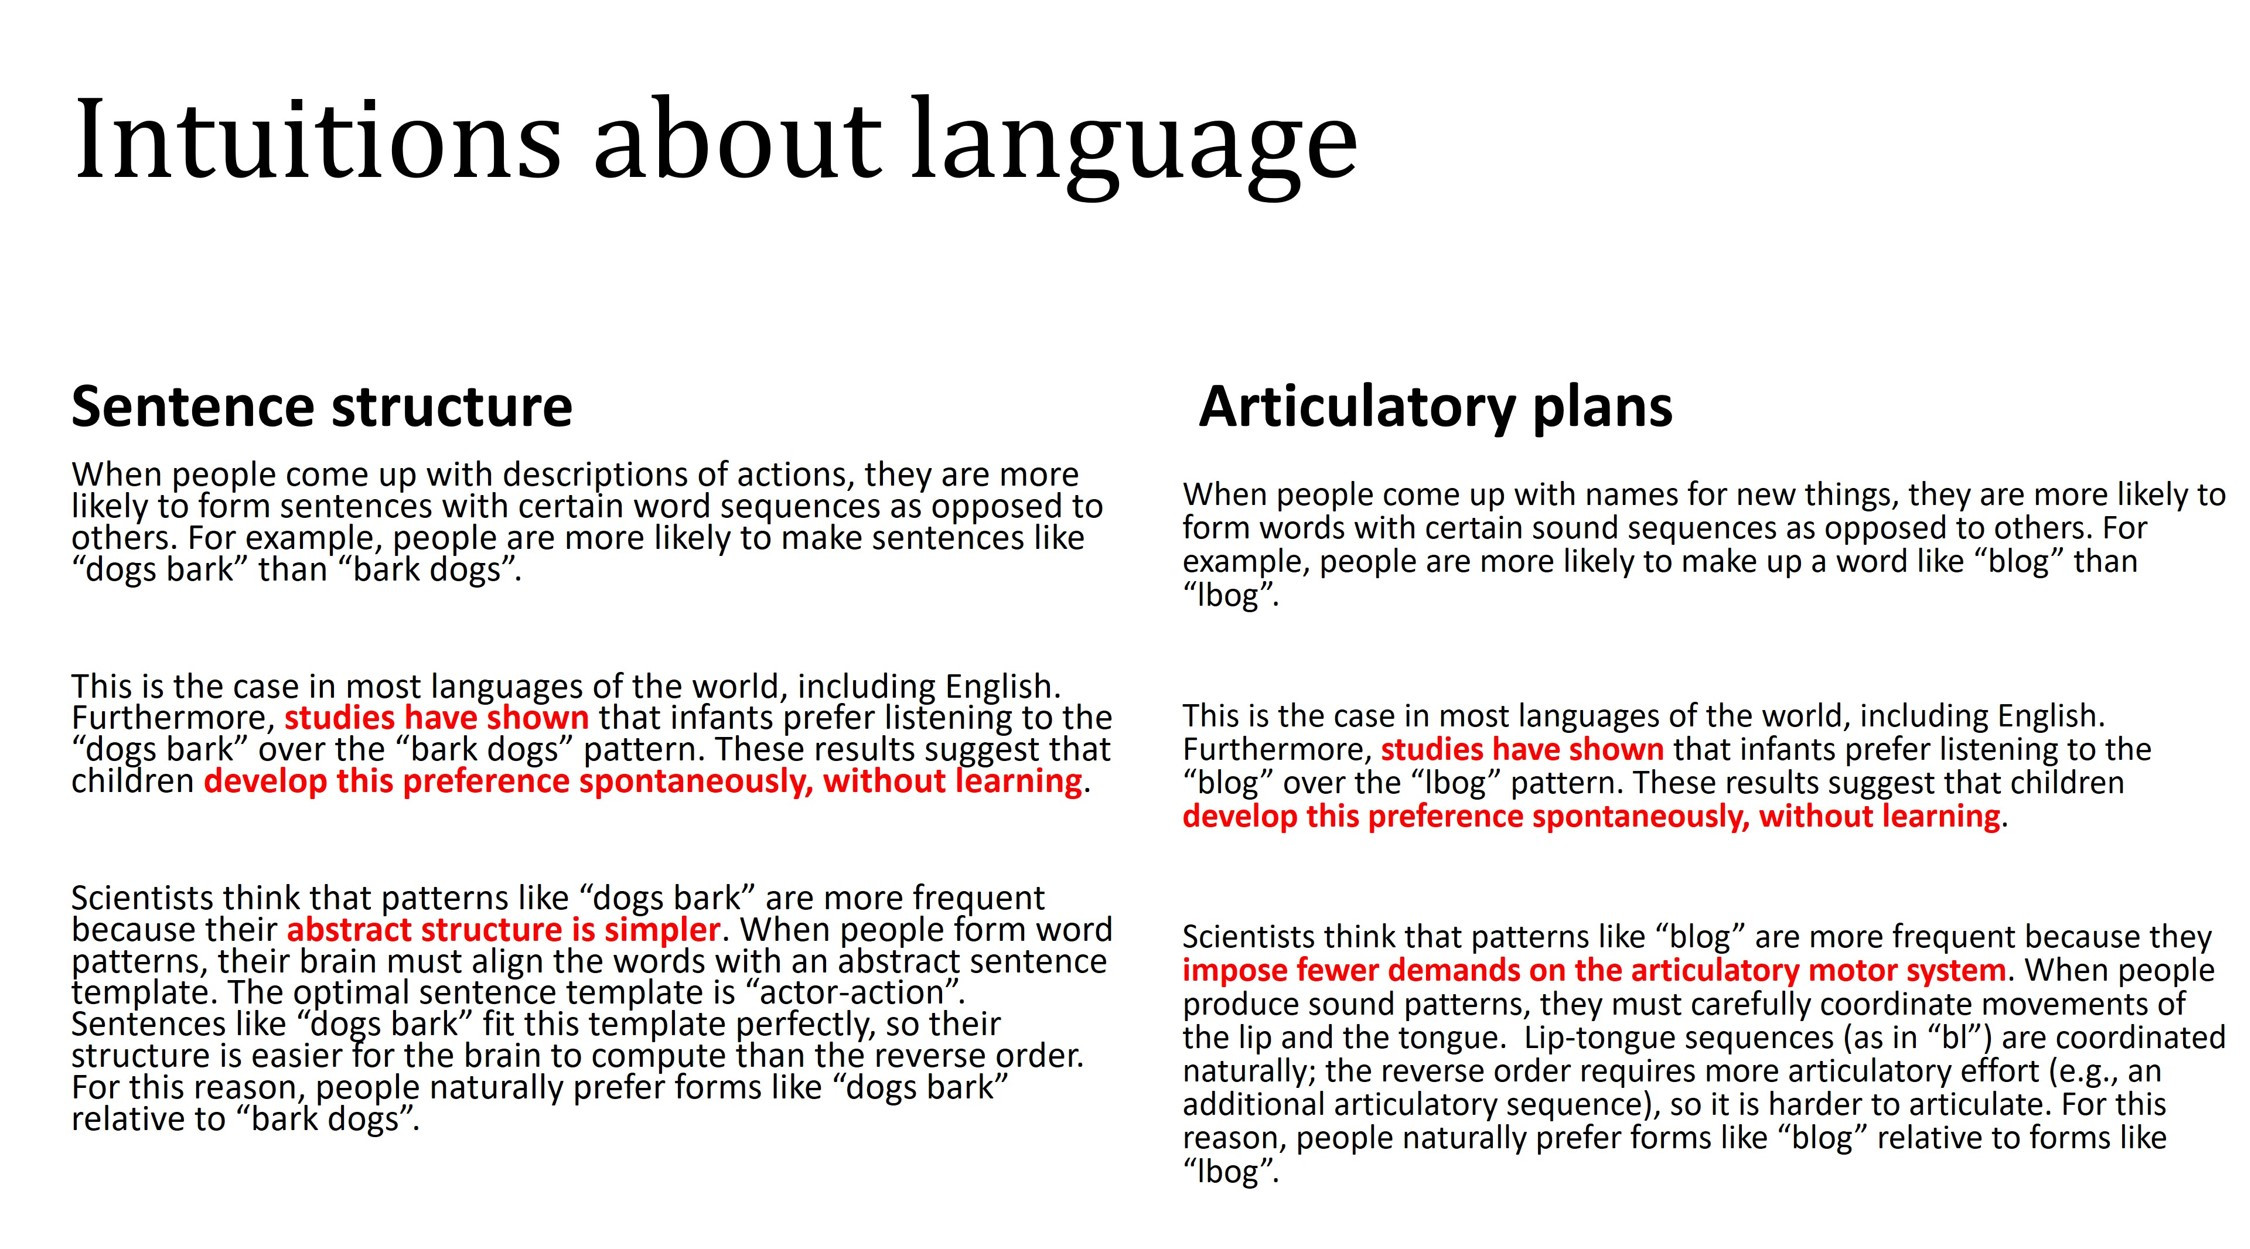
\includegraphics[width=\textwidth,keepaspectratio]{figures/berent_figure1a.jpg}
    \caption{}\label{fig:figure1a}
    \end{subfigure}\medskip\\
    \begin{subfigure}{\textwidth}
    \centering
    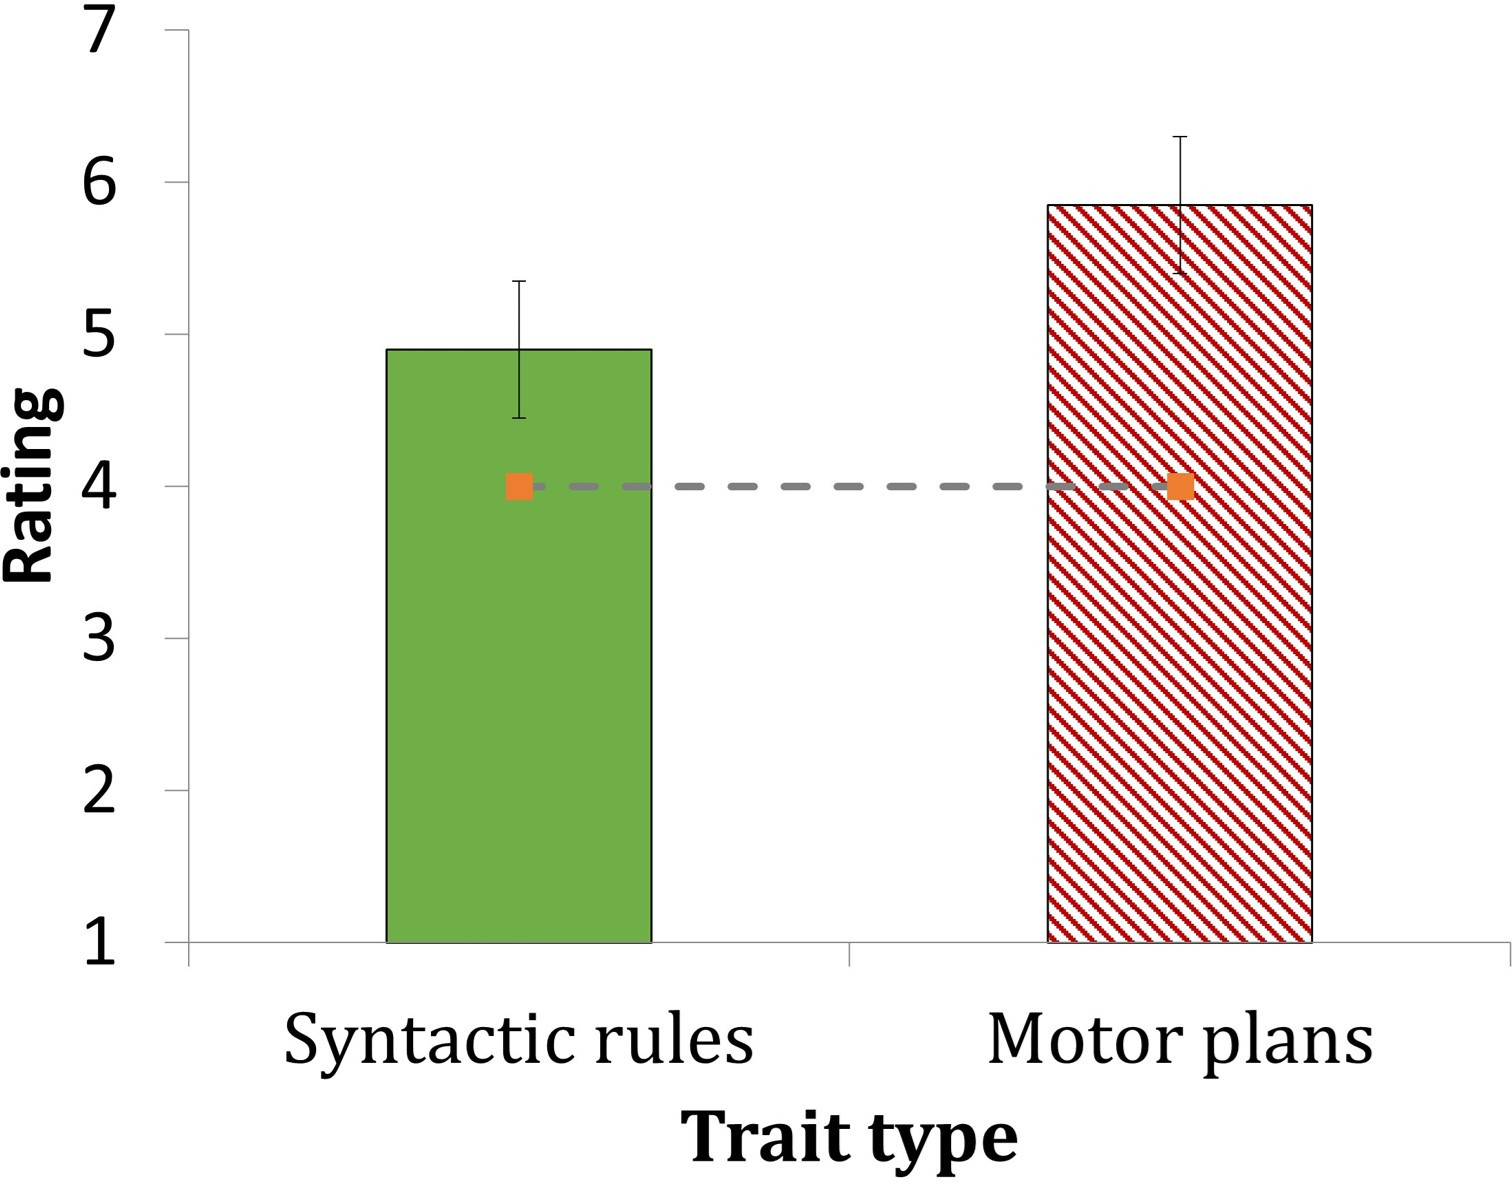
\includegraphics[width=.5\textwidth,keepaspectratio]{figures/berent_figure1b.jpg}
    \caption{}\label{fig:figure1b}
    \end{subfigure}
    \caption{Laypeople’s intuitions about the innate aspects of language (from \cite{berent2019people}).  
             Panel A illustrates the materials; Panel B plots the results.}
    \label{fig:figure1}
\end{figure}

Our troubles with innateness, then, are selective: people are biased to assume that knowledge cannot be innate. And if people reject innate knowledge, then it stands to reason that the notion of innate knowledge of language ought to be difficult for people to grasp.

\section{Why do we shun innate knowledge?}

To understand the scope of our troubles with UG, it is worth considering why people are biased in this particular fashion -- why they reject innate knowledge. The ``why'' question matters because, earlier, I’ve suggested that some scientific proposals are inherently difficult for the human mind -- they are hard because they violate principles of core knowledge.

This, however, may not necessarily be the case for Empiricism. Indeed, Empiricism can arise for many other reasons. Perhaps it is our experience with schooling that makes us expect knowledge to arise from learning. Or perhaps it is our fear of moral determinism and the dangers of social discrimination that leads us to reject Rationalism \citep{pinker2004blank}. People could also embrace Empiricism because they suffer from ``instinct blindness'' \citep{cosmides1994origins} or ``mindreading blindness'' \citep{carruthers2020mindreading}.

These proposals can certainly contribute to our troubles with innateness, and they are each justified in their own right. What they fail to explain, however, is the selectivity of our intuitions: why we specifically reject innate knowledge, yet remain open to the innateness of other psychological faculties, even though they, too, are learned (e.g., motor skills, like skating), are arguably more socially worrisome (e.g., emotions like aggression) and are equally amenable to the limits of instinct blindness and the shortcomings of mindreading.  

To explain why the notion of innate knowledge is especially difficult -- more so than any other forms of psychological innateness -- we need to invoke two intuitive psychological principles that are rooted in core knowledge: intuitive Dualism, and Essentialism \citep{berent2020blind,berent2021canwe}. Here, I briefly explain how these principles conspire to elicit resistance to innate knowledge. I will next explain what’s wrong with this reasoning. Finally, I will show how these biases are linked to core knowledge.

\subsection{A perfect Empiricism storm}
Empiricism, I suggest, arises from the collision between two intuitive principles: Essentialism and Dualism. Each of these principles are tacit -- they operate largely without conscious awareness, and as such, they should not be confused with the philosophical notions by the same names. And yet, these biases demonstrably interfere with reasoning.

Essentialism is that tacit belief that living things are what they are because of some innate immutable essence that they acquire from their biological parent \citep{keil1986acquisition,gelman2003essential}. Children, for instance, believe that a doggy is brown, like its mother, because of some tiny piece of matter that the doggy inherited from its mother \citep{springer1991early}. Per Essentialism, then, what’s innate lies deep within the body \citep{springer1991early}.

Dualism, on the other hand, is an intuitive belief that leads people to consider the mind as ethereal, distinct from the body \citep{bloom2005descartes}. And knowledge, quintessentially ``mental'', appears utterly ethereal. This belief is evident in many previous studies, suggesting that intuitions about knowledge dissociate, depending on whether the condition targets a person’s mind or the body. When asked to consider a scenario that duplicates one’s body, people assert that the replica will maintain the donor’s physical traits, but not their knowledge (e.g., \cite{hood2012children}). But when a manipulation targets only the mind (e.g., the afterlife), here, it is the donor’s knowledge that is most likely to persist (e.g., \cite{bering2004natural}). These dissociations suggest that knowledge is considered ethereal, in line with Dualism.

The Empiricist bias arises from the tension between Dualism and Essentialism (\figref{fig:figure2}). Recall that essentialism mandates that what’s innate lies in the body; Dualism, however, mandates that the mind is ethereal. It thus follows that the stuff of the mind cannot be innate. And since people consider knowledge a mental state, i.e., ethereal, the notion of innate knowledge -- of language or otherwise -- seems impossible, an oxymoron. 

\begin{figure}
    \centering
    \includegraphics[width=0.8\textwidth,keepaspectratio]{figures/berent_figure2.jpg}
    \caption{How Dualism and Essentialism conspite to beget Empiricism. }
    \label{fig:figure2}
\end{figure}

Recent results from my lab bear this theory out by showing that (a) people link innate traits to the body; (b) they consider knowledge ethereal; and (c) that intuitions about innateness and embodiment are linked \citep{berent2021can,berent2020essentialist,berent2021empiricism,berent2021essentialist,berent2021public,berent2021true}.

\subsection{It’s our logic that is faulty\ldots}

Suppose this theory is right, and intuitive psychology indeed biases people towards Empiricism. What’s the big deal? Are people actually wrong to endorse Empiricism? 

Given that the ``innateness wars'' are very much ongoing among scholars, this question is difficult to decide. If scholars cannot decide ``UG or not UG'', how can we qualify laypeople’s intuitions as right or wrong?

Obviously, we cannot. Innateness is ultimately an empirical question, and if the empirical facts are contentious, then we cannot determine whether laypeople’s judgments are wrong.  The real problem with laypeople’s intuitions, however, isn’t in the specific answer they arrive at (i.e., Empiricism). Rather, it is the logic that guides them that is problematic. 

Laypeople assume that (a) ``if it’s in the body, it’s likely innate''. This is obviously false -- many embodied traits are learned or emerge from experience (e.g., a scratch, Paris is the capital of France, etc.). People also assume (b) ``knowledge is ethereal, i.e., disembodied''. This, too, has no basis in science. And if intuitions about innateness are driven by such faulty assumptions, then the conclusions that they support are highly suspect. It’s the logic of innateness intuitions, then, that is faulty.

\section{Are we natural Empiricists?}\label{berent-section-4}\largerpage

Let’s stop to take stock of the argument thus far. I’ve argued that (a) Some scientific questions are hard because they violate principles of core knowledge; and (b) Innate knowledge, generally, and UG, specifically, is a question that is difficult for people to grasp, as the principles that guide reasoning are faulty. But how do these faulty assumptions arise -- do they emerge from principles of core knowledge? To rephrase the late Lila Gleitman, is Empiricism innate?

Gleitman was obviously joking. There is no reason to assume that Empiricism, or its purported instigators -- Dualism and Essentialism -- are innate; it is indeed difficult to see what selective advantage they might confer. But while Dualism and Essentialism are not directly innate, they could very well arise from an interaction between innate systems of core knowledge.

Essentialism could plausibly be linked to a number of distinctions that specifically can help identify living things as such, including notions of agency \citep{setoh2013young} and the distinction between artifacts and plants \citep{wertz2014selective}. And indeed, Essentialist thinking has been shown to arise spontaneously, even when participants’ culture attributes innate physical traits to social and cultural interactions \citep{astuti2004constraints}.

Dualism, in turn, has been linked to the interaction between knowledge systems. Core knowledge systems are early, putatively innate principles that guide reasoning in specific domains, such as Intuitive Physics, numerical cognition, intuitive biology and theory of mind \citep{spelke2007core}. Two of these systems of core knowledge could lead to Dualism: Intuitive Physics and Theory of Mind \citep{bloom2005descartes}. 

Briefly, Intuitive Physics maintains that objects can only interact by contact, and in the ``eyes'' of core physics, one’s body is just like a physical object. Yet Theory of Mind leads us to attribute people’s behavior to their mental states -- to their beliefs, knowledge and goals. 

\begin{figure}
    \centering
    \includegraphics[width=0.8\textwidth,keepaspectratio]{figures/berent_figure3.jpg}
    \caption{How Dualism arises from Intuitive Physics and Theory of Mind.}
    \label{fig:figure3}
\end{figure}

The problem, of course, is that what Theory of Mind suggests -- that invisible mental states can cause one’s body to move -- violates Intuitive Physics. The collision between the two systems might result in tension. To resolve the dissonance, people might assume that those invisible mental states are ethereal, rather than physical. And this is how Dualism emerges (\figref{fig:figure3}). 

Recent results from autistic individuals support this proposal \citep{berent2022autism}. Autism is known to compromise Theory of Mind. So, if Theory of Mind begets Dualism, then, compared to neurotypicals, autistic people ought to be less Dualist (and instead, lean towards Physicalism -- they should view the body and mind as alike). And if Dualism further begets Empiricism, then autistic people should also veer away from Dualism and towards nativism. This is exactly what was found.

Thus, while it is unlikely that Dualism and Essentialism are innate, they may be nonetheless rooted in core knowledge. And if the UG hypothesis violates core knowledge, then it is little wonder why people consider this hypothesis unlikely. 

To be clear, the question of whether Dualism and Essentialism are each rooted in core knowledge remains wide open; it is also unknown whether these two biases are universal, and whether they universally beget Empiricism; each of these steps is an open scientific question that requires much more research. As such, the theory advanced here remains partly speculative. Nonetheless, there are reasons to expect that (a) Dualism and Essentialism emerge in humans quite generally; (b) they are rooted in core knowledge; and (c) they are responsible for our Empiricist intuitions. If so, our troubles reasoning about innate knowledge could be principled.

\section{Scholars aren’t immune from the claws of Empiricism}

While the question of why people are Empiricist is still open, it seems safe to conclude that laypeople are Empiricist -- this is certainly so for Western participants, and the empirical support for this conclusion is sound. So, inasmuch as laypeople are biased, and scholars are people, scholars may not be immune from this bias either. 

There is some evidence that indeed, they are not. I will first consider experimental results documenting an Empiricist bias among scholars; I will then consider some intuitions about phonology and how they fare against scientific evidence. To be clear, these results are insufficient to establish that phonologists are biased. But they certainly suffice to urge scholars to exercise greater caution.

\subsection{``Mind scientists'' underestimate core knowledge}
\begin{sloppypar}
To evaluate scholars’ reasoning about innateness, \citet{wang2019empiricism} asked a large group of academics ($N=400$) to evaluate the origins and onset of a number of psychological traits. Some of the questions captured sensory traits (e.g., How come Alex can see/hear?); others captured aspects of core knowledge (e.g., How come Alex thinks that hidden objects are still there?) and some consisted of knowledge that is clearly learned (e.g., reading). 
\end{sloppypar}

Results showed that, when it comes to core knowledge, scholars grossly overestimated the role of learning, and thought these traits emerge far later in life than they demonstrably do. Shockingly, this was also the case for ``mind scientists'' -- those that work in linguistics, psychology and neuroscience ($N=200$). While \citet{wang2019empiricism} did not assess the source of those intuitions, their results make it clear that ``mind scholars'' do lean towards Empiricism.

To reiterate, these results do not establish that scholars reject UG, and they certainly don’t show that if one rejects UG, then this position reflects an intuitive bias. Still, in light of the linguistic biases detected in laypeople (see \figref{fig:figure1}), certain assumptions about language ought to be particularly alluring to scholars. We now review laypeople’s intuitive understanding of phonology and compare it with some of the ``received wisdom'' amongst linguists. 

\subsection{Phonological intuitions: ``It’s all in my body''}

Laypeople, recall, believe that innate traits must be patently embodied. So, to the extent that language seems to exhibit some common structural regularities, those putative innate tendencies ought to arise from physical, rather than cognitive, constraints. The leap from ``language universals'' to ``physical causes'' (e.g., articulatory, auditory) is especially alluring for phonology, where cross-linguistic regularities are well attested (e.g., \cite{greenberg1966universals}), and physical (articulatory, auditory) limitations are patent to introspection. 

For example, it is well established that (a) syllables like \textit{blog} (with obstruent-sonorant onsets) are far more frequent across languages than \textit{lbog} (with the reverse sequence), and that languages that tolerate the latter (\textit{lbog}-type) syllables tend to also manifest the former (e.g., \textit{blog}-type syllables; \cite{greenberg1978some}). Moreover, similar preferences arise in the behavior of individual speakers (e.g., \cite{berent2013phonologicalb}). It is also patently evident that (b) language production is subject to articulatory limitation, and that \textit{blog}-type syllables are preferred on articulatory and auditory grounds \citep{mattingly1981phonetic,wright2004review}. A critical scientific question is whether the physical limitations (b) are the direct cause of the typological and behavioral observations (a). 

\begin{figure}
    \centering
    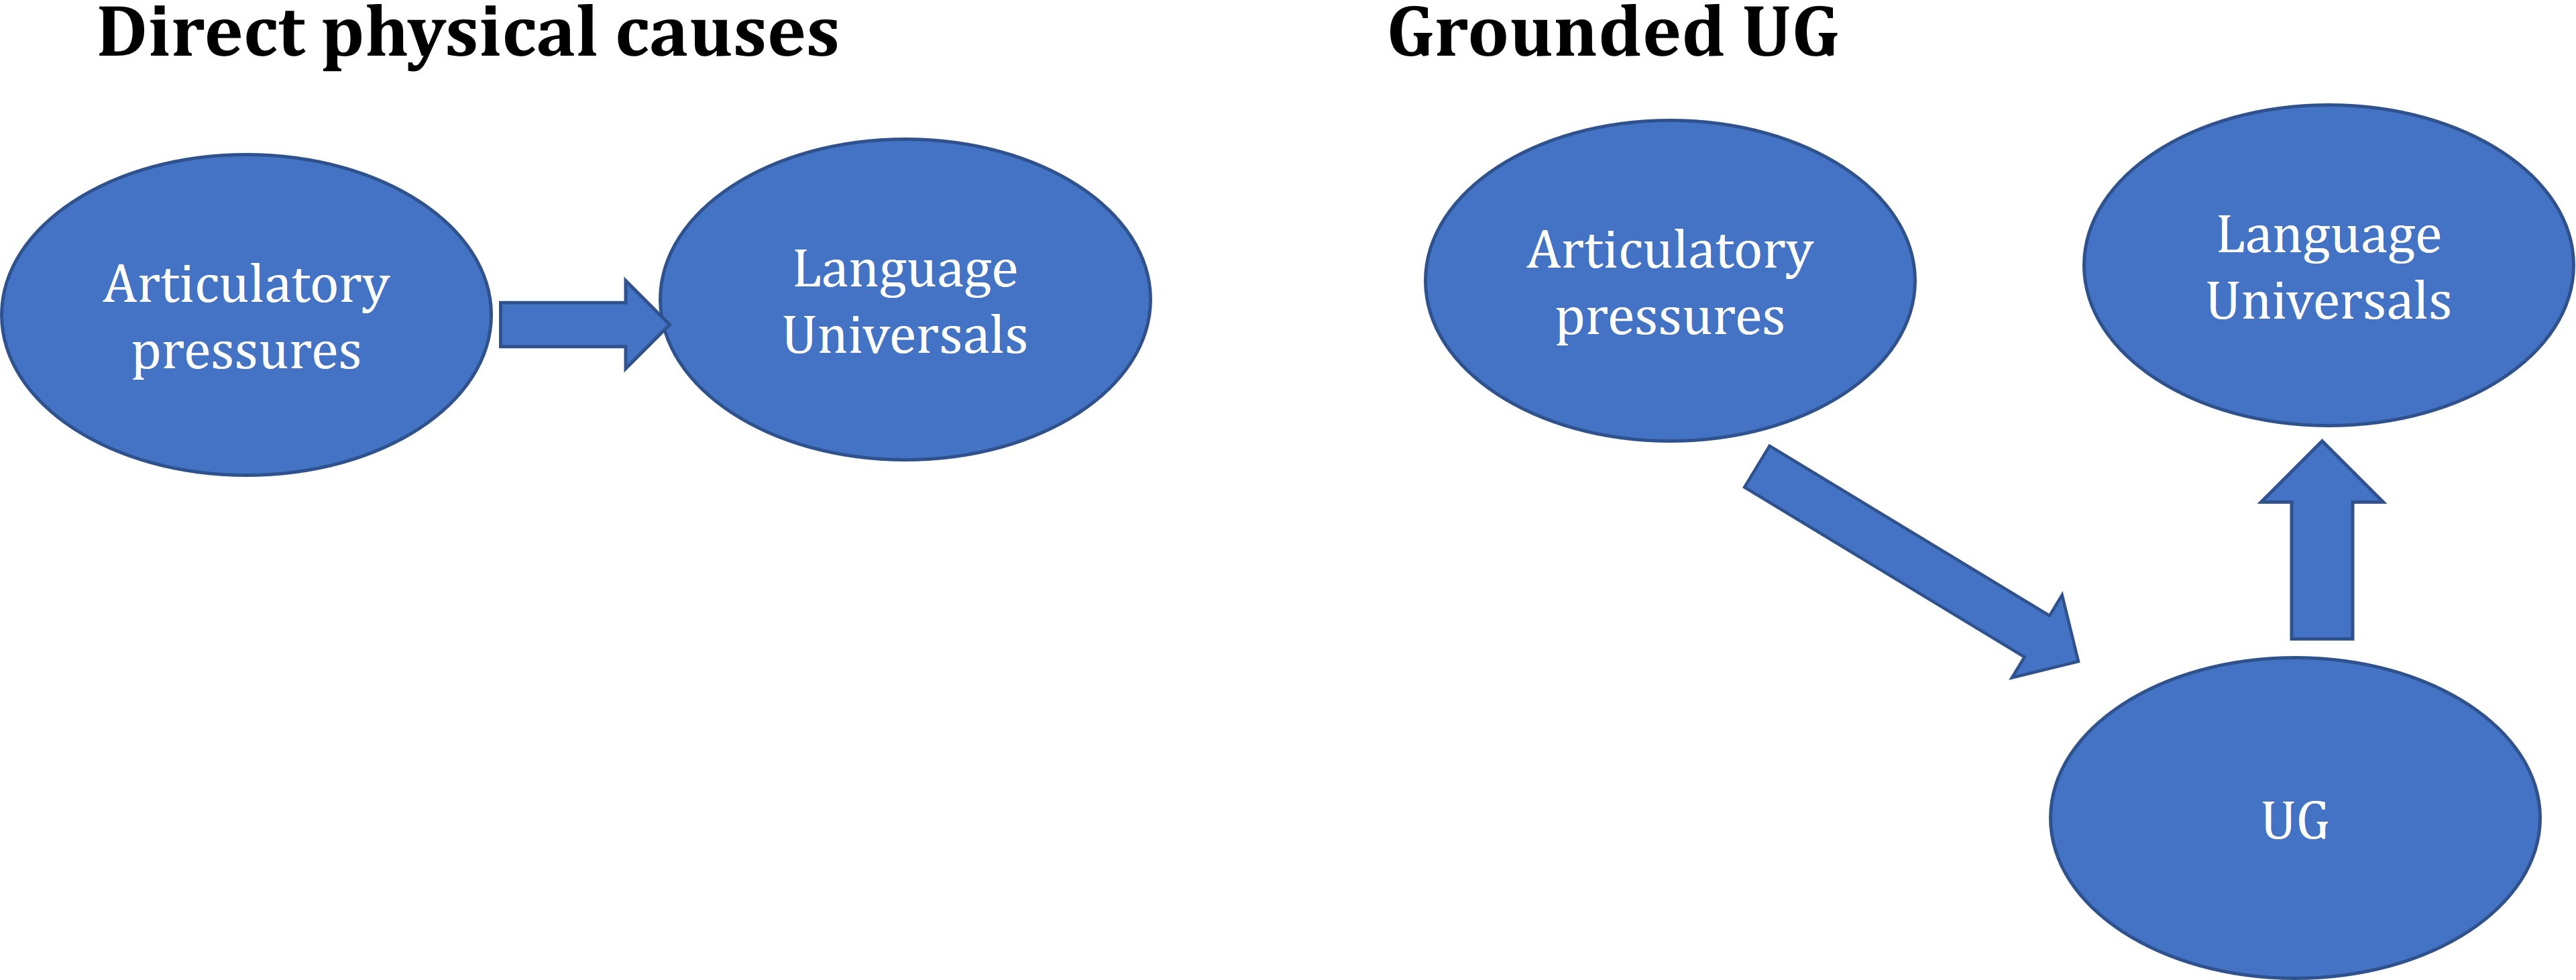
\includegraphics[width=\textwidth,keepaspectratio]{figures/berent_figure4.jpg}
    \caption{Two competing accounts of phonology.}
    \label{fig:figure4}
\end{figure}

\begin{sloppypar}
The causation is uncertain because, logically speaking, the correlation between these two facts -- (a) and (b) -- can also arise from other sources. In particular, it is conceivable that the human preference for \textit{blog} arises not from the physical causes directly (from (b)), but rather from a third cause -- from some universal linguistic principles, UG (\figref{fig:figure4}). One can further speculate that those UG principles acquire this particular shape because they have been constrained by physical limitations in ontogeny and phylogeny -- they are ``grounded'' in the sensorimotor system. And yet, the linguistic preferences evident in behavior could still be caused, in part, by UG \citep{berent2013phonologicala}. Put simply, the correlation between physical limitations and linguistic preference (b) does not necessarily imply causation.
\end{sloppypar}

A priori, one could, of course, challenge the ``UG grounding'' hypothesis using arguments from parsimony: if physical constraints can explain the phonological facts, then the assumption of other sources is unnecessary (i.e., unparsimonious). But arguments from parsimony are hardly decisive. In fact, since evolution is a tinkerer, not an inventor \citep{jacob1977evolution}, unparsimonious biological systems are only expected. Accordingly, if discussions of UG are to rely on arguments from parsimony, then those arguments ought to be a weapon of last resort -- it is the empirical evidence that ought to win the day. 

And yet, few phonologists bother to differentiate, let alone adjudicate, between these competing hypotheses. For example, Fitch, Hauser and Chomsky have famously asserted that ``Much of phonology is likely part of FLB, not FLN'' \citep{fitch2005evolution}, but they bring only scant arguments in support of this conclusion. The lack of interest in the causal role of the motor system is particularly surprising given that the notion of ``grounded phonology'' is quite influential in modern phonology \citep{archangeli1994grounded,hayes2004phonetically}.

Why phonologists often assume that the correlation (between language universals and the sensorimotor system) implies causation is a question I cannot decide here. Instead, I describe in detail one recent piece of experimental evidence that calls this common practice into question \citep{berent2023phonetic}. 

\subsection{Science counters our phonological intuitions: Evidence from TMS}

To dissociate the causal role of the motor system from phonological preferences, my colleagues and I used Transcranial Magnetic Stimulation (TMS) -- a method that perturbs (either increases or decreases) activity in specific brain areas by applying an electromagnetic current \citep{rossi2021safety}.  

A large literature, including many TMS studies, has shown that phonetic categorization relies on the articulatory motor system. Thus, the perception of labial sounds is selectively disrupted when the lip articulatory motor system is stimulated, whereas the identification of coronal sounds is selectively disrupted by stimulating the tongue. In both cases, these effects obtain regardless of whether the relevant articulator is stimulated using TMS \citep{d2012role, d2009motor, mottonen2009motor,smalle2015dissociating}, or mechanically (e.g., by having participants bite on the lips vs. tongue, e.g., \cite{bruderer2015sensorimotor}; see also \cite{berent2020speech}). 

These results make it clear that phonetic categorization relies on motor simulation: to perceive a labial, people must tacitly simulate the articulatory process of producing a labial sound. Accordingly, when the process is disrupted (mechanically, or by TMS), identification is altered selectively.  

All this shows that speech perception engages the articulatory motor system, just as our intuitions suggest. But there is a big caveat: the results presented so far concern phonetic categorization. And what is true for phonetics may not necessarily ``scale up'' for phonology. Our intuitions, of course, suggest it must. But as we should now know, what our intuitions say ought to be taken with a very large grain of salt. Better yet is to confront them directly using science. And so, we did.

In a series of experiments, we compared the effect of TMS on two tasks: phonetic and phonological \citep{berent2023phonetic}. As participants performed the task, we applied TMS to either the brain motor area that controls the lip (the Orbicularis Oris, OO), or to a part of Broca’s area (the Pars Triangularis, PT). 

We reason that, if the computation in each task relies on motor simulation, performance ought to be more strongly perturbed by stimulating the OO than the PT. But if the computation recruits abstract linguistic principles, then stimulating the PT ought to play a greater role; this is in line with past research suggesting that phonological computation of syllable structure engages the PT \citep{berent2014language}.

The phonetic task asked participants to identify a speech sound that was ambiguous with respect to its voicing -- either labial (in between\textit{ba}and \textit{pa}) or coronal (in between \textit{da} and \textit{ta}). The logic is that, if motor simulation plays a role, then it ought to affect the perception of all features associated with a given phoneme, including voicing. Of interest is whether the perception of voicing will differ, depending on the congruence between the sound’s place of articulation (labial or not) and the stimulated area (controlling the lips or not, i.e., OO vs. PT). 

Results suggested that it did, as the stimulation of the OO had opposite effects on labials and coronals. For the coronal sound, OO stimulation increased ``voiced'' (i.e., \textit{da}) response (relative to the PT). For the labial sound, by contrast, OO stimulation tended to attenuate ``voiced'' (i.e., \textit{ba}) responses (relative to the PT). So far, these conclusions replicate and extend past research showing that the speech-motor system has a causal role in phonetic categorization.

The critical question concerns its role in phonological processing. To find out, we applied the same TMS manipulation to a phonological task. Here, we presented participants (English speakers) with two types of unattested monosyllables (e.g., \textit{bnif} vs. \textit{lbif}) along with their disyllabic counterparts (e.g., \textit{benif} vs. \textit{lebif}) -- the task was to count the number of syllables (one/two). 

Results showed that, in the syllable count task, the stimulation of the PT perturbed performance more than the OO: it promoted a bias to perceive all stimuli (monosyllables or disyllables) as disyllabic. The bias is only expected if the PT plays a causal role in the computation of syllable structure. If it does, then disrupting the PT ought to disrupt sensitivity to syllable structure; consequently, sensitivity to syllable structure ought to decline, and bias ensues. This is precisely what we found.

To summarize (see \figref{fig:figure5}), these results suggest that phonetic categorization relies on the speech-motor system, just as our intuitive psychology suggests. But the phonological computation of syllable structure does not: it relies on Broca’s area (PT) more heavily than the motor system. Moreover, this effect of Broca’s area is causal: when the PT is disrupted, the computation of syllable structure declines accordingly.

\begin{figure}
    \centering
    \includegraphics[width=\textwidth,keepaspectratio]{figures/berent_figure5.jpg}
    \caption{Graphic summary: phonetic categorization relies on motor simulation (by the OO), whereas the phonological combinatorial computation of syllable structure is abstract, and engages Broca’s area (the PT) (from \cite{berent2023phonetic}). }
    \label{fig:figure5}
\end{figure}

This conclusion flies in the face of our intuition that the dispreference of \textit{lbog} is caused by motor difficulties alone. To be clear, these results do not specifically speak to whether the ban on \textit{lbog} arises from rules, nor do they tell us about the origins of those rules -- innate or learned. Thus, these results are moot with respect to the question of UG. 

Still, a large literature in phonology and psychology interprets the undeniable correlations between phonological universals and articulatory constraints as causation (e.g., \cite{hayes2004phonetically}). This study suggests that this assumption ought to be revisited. In line with this conclusion, other results suggest that the restriction on onset structure is present at birth (well before infants can articulate such syllables; \cite{gomez2014language}) and it also survives a mechanical form of articulatory suppression \citep{berent2022phonology}. 

At yet a broader level, research from my lab has shown that some phonological restrictions (a) rely on abstract algebraic rules (rather than statistical regularities alone, e.g., \cite{berent2002scope,gervain2012binding}); and (b) they apply amodally~-- speakers spontaneously project their knowledge of spoken language to signs \citep{berent2021amodal,berent2016double,berent2020knowledge,berent2021infants,berent2023phonetic}. 

Thus, the presumption that ``phonology is all in my body'' is false: the correlation between phonology and articulation doesn’t imply causation. And yet, the presumption of causation is prevalent. To the extent scholars maintain this bias despite evidence to the contrary, the possibility of a bias ought to be considered. 

\section{Why is UG so hard?}

Why, then, is UG so difficult for us to grasp -- arguably, even for scholars? I think the answer to this question becomes clearer when we place our troubles within a broader context. Indeed, UG is hardly the only ``hard'' question. Many scientific theories can be perfectly coherent, and yet, they are difficult for people to grasp.

Quantum physics and evolutionary biology are notorious examples. Concepts in these fields are amenable to formal description, and yet, they are difficult for us to comprehend. Even notions such as ``gravity'' and ``electromagnetism'' are hard for laypeople -- it is difficult to appreciate that forces can apply at a distance  \citep{chomsky2015kind,shtulman2017scienceblind}. These proposals are perfectly coherent, but they are not fully intelligible: these are notions that people struggle to grasp intuitively. This difficulty likely arises because these scientific concepts violate principles of core knowledge \citep{shtulman2017scienceblind}. 

Consider, for example, Intuitive Physics. Young infants -- indeed, newborns and nonhuman animals -- possess an early understanding of what objects are and how they behave \citep{mascalzoni2013cradle,regolin1995perception,vallortigara2021born}. They know that objects are cohesive entities that interact only by contact \citep{spelke1992origins}. So, when they see an impossible event, such as contactless interaction between two moving balls, infants are demonstrably surprised \citep{mascalzoni2013cradle}. And, if we come to the world expecting physical causation to require contact, it is no wonder that, when physical science shows us that forces can operate at a distance (e.g., gravity), we are baffled. The concept of contactless physical causation is perfectly coherent, but it violates Intuitive Physics.  For this reason, the notion of ''contactless causation'' is hard. 

I believe the same applies for UG. As we have seen (in \sectref{berent-section-4}), the notion of ``innate knowledge'', generally, likely violates Essentialism and Dualism -- biases that are rooted in core knowledge. And scientific theories that violate core knowledge are hard for us to grasp. Accordingly, core knowledge could well explain our troubles with UG.

\section{Conclusions}
In this piece, I sought to determine why the UG question is such a difficult problem for scholars. I’ve argued that the problem isn’t in the question itself -- there is nothing incoherent about asking whether knowledge~-- of language or otherwise~-- is innate. And yet, the possibility of innate knowledge seems difficult for us to grasp. 

New evidence suggests that laypeople are systematically biased against this possibility, and there is evidence that their biases are rooted in core cognition. These results open up the possibility that the difficulty with UG arises for the same reasons that people struggle to reason about gravity, electromagnetism and natural selection: these scientific proposals violate principles of core knowledge. There is indeed preliminary evidence to suggest that ``mind scientists'' systematically underestimate the role of core knowledge, and some anecdotal evidence to suggest that articulatory explanations of phonology are alluring. How this bias arises, and whether it is linked to core knowledge cannot be determined here. This possibility, however, cannot be ruled out.

Still, the possibility that scholarly discussions of UG are biased hardly means destiny -- that the UG question cannot be scientifically evaluated. This conclusion doesn’t follow because people are equipped with systems of rational reasoning. So even if intuitive psychology engenders bias, we can still put checks and balances on our intuitive biases, just as we do in many aspects of math, physics and biology. But if such biases exist, then recognizing them might be a necessary first step to reining them in. And this is precisely why I’m writing this piece.

Evidently, the view of human nature I advance does not accord with Dan’s current position. But the pursuit of human nature is a passion we share in common, and I have embarked on this path guided, in part, by his teachings. 

A certain personal anecdote might serve as an illustration. As noted, Dan was my only linguistics teacher -- I took with him one and a half classes; the ``half'' was a seminar in phonology, cut short by the birth of my son. But notwithstanding the challenges of fitting the nine-month pregnancy within the confinements of the seminar chairs, I was there pretty much until the last day. On my way to the hospital, one November night at 2:30 am, I saw a light up at the Cathedral of Learning, where Dan’s office was. Recognizing his work ethic, legendary among the impressionable students, I couldn’t help wondering in between contractions: is it really Dan up there? What is he writing? This is to show that, when I think of nativism, Dan has been in my mind often, and in more ways than one. 

\printbibliography[heading=subbibliography,notkeyword=this]

\sloppy
\end{document}
